\chapter{Complex Attosecond Transient-absorption Spectroscopy}
\label{chap:CATS}

\section{Introduction}
\label{sec:intro_cats}

As seen in Chapter \ref{chap:ATS}, a rich amount of information can be extracted from ATS experiments.  Specifically, dynamics such as light-induced states and strong-field ionization of  excited states induced by a dressing field can be deduced from the change in photoabsorption cross section.  However, these experiments are limited by the fact that they only have access to the imaginary part of the complex refractive index of the medium of interest. There should also be a corresponding change in the real part of the complex refractive index that remains unobserved.  In this Chapter, the techniques introduced in Chapters \ref{chap:two_source} and \ref{chap:refractive_index} are extended to measure both parts of the complex refractive index in the experiments performed in Chapter \ref{chap:ATS}.  This new method to measure the change in the complex refractive index induced by a dressing field will be referred to as Complex Attosecond Transient-absorption Spectroscopy (CATS).


\section{Theory}
\label{sec:cats_theory}

In ATS experiments, such as those described in Chapter \ref{chap:ATS}, the dynamics induced by a dressing field is imprinted upon the photoabsorption cross section and, macroscopically, the optical density (OD) of the sample \cite{wuTheoryStrongfieldAttosecond2016,geneauxromainTransientAbsorptionSpectroscopy2019}.  Measuring a change in the OD of the sample yields a rich amount of information, however it does not represent a direct measurement of all the of the changes induced in the sample. 

To see why this is the case, consider the following scenario: a gas of atoms with density $\rho$ that is interacting with a two-color field $\mathcal{E}(t)$ consisting of an XUV APT and an IR dressing pulse that is of moderate intensity and time delayed from the XUV APT. Moderate intensity in this particular case means that the dressing field is not strong enough to excite or ionize the ground state of the atom, but it is strong enough to further excite or ionize once the atom has been excited by the XUV APT pulse.  The goal is to characterize the the evolution of the electric field as it propagates through this gas medium along a direction $z$. Macroscopically, this can be described by Maxwell's wave equation (MWE), and in a frame that moves at the speed of light the frequency-domain MWE in cylindrical coordinates under the slowly evolving wave approximation is given by
\begin{equation}
	\label{eqn:MWE}
	\nabla_{\perp}^{2}\tilde{\mathcal{E}}(\omega) + \frac{2i\omega}{c}\frac{\partial \tilde{\mathcal{E}}(\omega)}{\partial z} = -\frac{\omega^2}{\epsilon_0 c^2}\tilde{P}(\omega)
\end{equation}
where $\tilde{\mathcal{E}}(\omega)$ is the two-color electric field in the frequency-domain $\omega$ and $\tilde{P}(\omega)$ is the polarization\footnote{This is neglecting the polarization contribution from free electrons that have been ionized.  This is reasonable because we are assuming a moderate intensity of the dressing pulse, so this term is small and can be neglected unless higher intensities are used \cite{gaardeTransientAbsorptionReshaping2011}.} in the frequency domain \cite{jacksonClassicalElectrodynamics1999, brabecIntenseFewcycleLaser2000, wuTheoryStrongfieldAttosecond2016, gaardeTransientAbsorptionReshaping2011}. In order to solve for $\tilde{\mathcal{E}}(\omega)$, the polarization source term $\tilde{P}(\omega)$ needs to be calculated, and this is achieved by solving the TDSE for the single atom dipole moment $d(\omega)$.  This can be done in the single-active electron (SAE) approximation \cite{eberlyNumericalExperimentsStrong1992, schaferHighHarmonicGeneration1997}, and the dipole is calculated from the time-dependent acceleration $a(t)$ given by 
\begin{equation}
	a(t)=\frac{\diff^2 \braket{z}}{\diff t^2} = -\braket{\psi(t)|[\hat{H},[\hat{H},\hat{z}]]|\psi(t)}.
\end{equation}
The dipole $\tilde{d}(\omega)$ in the frequency-domain is related to the Fourier transform $\tilde{a}(\omega)$ of $a(t)$ by the relationship $\tilde{d}(\omega)=\tilde{a}(\omega)/\omega^2$.  Typically, in order to account for a finite dephasing time that naturally occurs a window function $W(t)$ is applied when Fourier transforming $a(t)$, and this results in
\begin{equation}
	\tilde{a}(\omega)=\frac{1}{\sqrt{2\pi}}\int_{-\infty}^{\infty}a(t)W(t)e^{i\omega t}\diff t.
\end{equation}
From this, it is now possible to calculate the macroscopic polarization $\tilde{P}(\omega)$ as 
\begin{equation}
	\tilde{P}(\omega)=g\rho\tilde{d}(\omega)=\frac{g\rho e}{\omega^2\sqrt{2\pi}} \int_{-\infty}^{\infty}a(t)W(t)e^{i\omega t}\diff t.
\end{equation}
where $\rho$ is the gas density and $g$ is the number of active electrons, which is typically 2 for rare gas atoms since there are two active electrons with the same $m=0$ quantum number.  Substituting this form of the polarization into equation \ref{eqn:MWE} and assuming the limiting case of a linear-response the MWE becomes
\begin{equation}
	\label{eqn:MWE_linear_resp}
	\begin{aligned}
		\frac{2i\omega}{c}\frac{\partial \tilde{\mathcal{E}}(\omega)}{\partial z} &= -\frac{\omega^2}{\epsilon_0 c^2} g\rho \tilde{d}(\omega)\\
		& = -\frac{\omega^2}{\epsilon_0 c^2} \frac{g\rho \tilde{d}(\omega)}{\tilde{\mathcal{E}}(\omega)}\tilde{\mathcal{E}}(\omega).
	\end{aligned}
\end{equation}
Furthermore, in this linear-response limit, it can be assumed that $\tilde{d}/\tilde{\mathcal{E}}$ is approximately constant during propagation through the medium \cite{wuTheoryStrongfieldAttosecond2016}.  This allows for a simple solution given by
\begin{equation}
	\label{eqn:E_solution_MWE}
	\begin{aligned}
		\tilde{\mathcal{E}}(\omega,z) &= \tilde{\mathcal{E}}_0 \exp\Bigg({\frac{i\omega\rho}{2\epsilon_0 c} \frac{g\tilde{d}(\omega)}{\tilde{\mathcal{E}}(\omega)} z}\Bigg)\\
		&=\tilde{\mathcal{E}}_0 \exp\Bigg({\frac{i\omega\rho g}{2\epsilon_0 c} \mathrm{Re}\bigg[\frac{\tilde{d}(\omega)}{\tilde{\mathcal{E}}(\omega)}\bigg]z}\Bigg) \exp\Bigg(- {\frac{\omega\rho g}{2\epsilon_0 c} \mathrm{Im}\bigg[\frac{\tilde{d}(\omega)}{\tilde{\mathcal{E}}(\omega)}\bigg]z}\Bigg)\\
		&=\tilde{\mathcal{E}}_0 \exp\bigg(-\tilde{\beta}(\omega)\frac{\omega}{c}z\bigg) \exp\bigg( i\tilde{n}(\omega) \frac{\omega}{c} z\bigg)
	\end{aligned}
\end{equation}
where the real $\tilde{n}(\omega)$ and imaginary $\tilde{\beta}(\omega)$ parts of the complex refractive index are given by
\begin{equation}
	\begin{aligned}
		\tilde{n}(\omega) &= \frac{g \rho}{2 \epsilon_0} \mathrm{Re}\Bigg[ \frac{\tilde{d}(\omega)}{\tilde{\mathcal{E}}(\omega)} \Bigg]\\
		\tilde{\beta}(\omega) &= \frac{g \rho}{2\epsilon_0} \mathrm{Im}\Bigg[ \frac{\tilde{d}(\omega)}{\tilde{\mathcal{E}}(\omega)} \Bigg] = \frac{\rho c}{2\omega}\sigma(\omega) = \frac{c \ln 10}{2\omega L} \mathrm{OD}(\omega),
	\end{aligned}
\end{equation}
and the relationship between the imaginary part $\tilde{\beta}$, the cross section $\sigma(\omega)$, and the optical density $\mathrm{OD}(\omega)$ is also shown for a medium length $L$.  This complex refractive index $\tilde{n} + i\tilde{\beta}$ describes the dispersion and absorption of the excited state of the gas medium in the presence of the IR dressing field.  In a typical ATS experiment, only the change in absorption due to the dressing field is measured through the $\dod$, and this can be written in terms of the dipole as 
\begin{equation}
	\label{eqn:dod_im_dipole}
	\dod(\omega) = \frac{g \omega \rho L}{\epsilon_0 c \ln 10}\Bigg( \mathrm{Im}\Bigg[\frac{\tilde{d}_{\mathrm{on}}(\omega)}{\tilde{\mathcal{E}}_{\mathrm{on}}(\omega)}\Bigg] - \mathrm{Im}\Bigg[\frac{\tilde{d}_{\mathrm{off}}(\omega)}{\tilde{\mathcal{E}}_{\mathrm{off}}(\omega)}\Bigg] \Bigg),
\end{equation}
where the subscripts on (off) refer to when the IR dressing field is present (absent).

As can be clearly seen, only the imaginary part of the dipole is measured in a typical ATS experiment by measuring the $\dod$, such as was described in Chapter \ref{chap:ATS}.  These experiments are only able to directly measure half of the total changes induced by the dressing pulse because they are blind to the change in dispersion that arises from the change in the real part of the refractive index due to the real part of the dipole.  For completeness, this change in real part of the refractive index is given by 
\begin{equation}
	\label{eqn:dn_re_dipole}
	\Delta n(\omega) = \frac{g\rho}{2 \epsilon_0} \Bigg( \mathrm{Re}\Bigg[\frac{\tilde{d}_{\mathrm{on}}(\omega)}{\tilde{\mathcal{E}}_{\mathrm{on}}(\omega)}\Bigg] - \mathrm{Re}\Bigg[\frac{\tilde{d}_{\mathrm{off}}(\omega)}{\tilde{\mathcal{E}}_{\mathrm{off}}(\omega)}\Bigg] 
	\Bigg).
\end{equation}
In order to directly measure the full complex refractive, and consequently both parts of the dipole, then a more advanced technique is required. 


\subsection{Direct Measurement}

To directly measure this expected change in the real part of the refractive index there are a few methods that can be applied.  One technique that is often used is an interferometric method to measure the change in refractive index as a phase shift between two arms of a Mach-Zehnder interferometer, and this concept was introduced in detail in Chapter \ref{chap:refractive_index}. In general, interferometric techniques are technically challenging in this wavelength range because of a lack of broadband and efficient optics and a high interferometric stability required by the relatively short wavelengths.  There are a few methods to overcome these challenges, and they generally can be divided into two different approaches: either splitting the XUV beam after it is generated (for example, with split mirrors \cite{nabekawaInterferometricAutocorrelationAttosecond2008, nabekawaInterferometryAttosecondPulse2013}) or generating two nearly identical XUV beams that can be interferred (for example, with a Michelson interferometer before generation of the XUV \cite{kovacevExtremeUltravioletFourierTransform2005}).  In Chapter \ref{chap:two_source}, it was shown how the later approach can be implemented using a SWPG that is able to control the relative phase of the two generated XUV beams.  Furthermore, in Chapter \ref{chap:refractive_index} it was demonstrated that this setup can be used to measure the refractive index of two different materials by measuring a phase shift between the two generated XUV sources over a broad energy range.  In that case, the phase shift induced by the sample was known \textit{a priori} because the ground state refractive index has been well characterized previously, and the excellent agreement between the extracted refractive index and the known refractive index demonstrated the validity of this technique.  

\begin{figure}
	\centering
	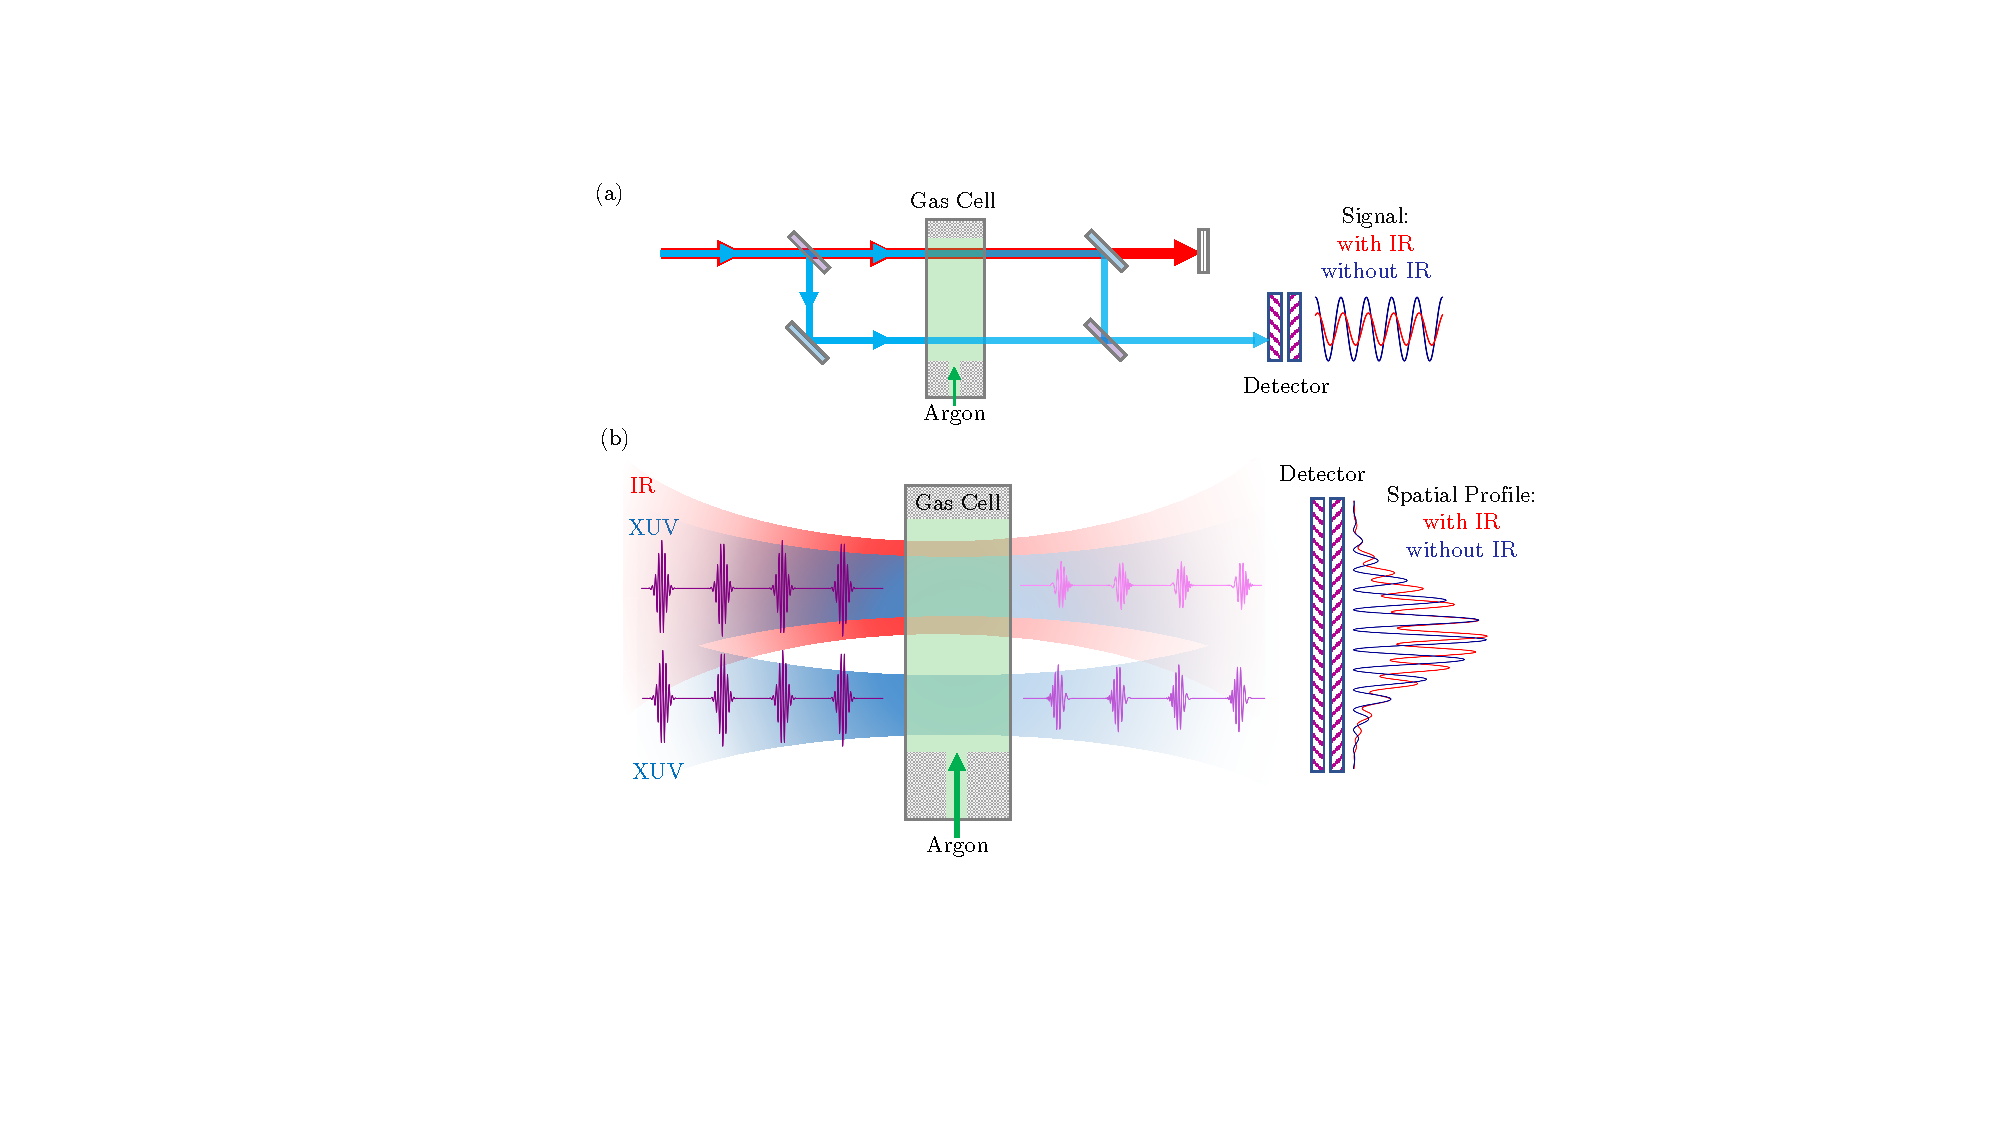
\includegraphics[width=1.0\textwidth]{figures/CATS/CATS_mach_zehnder.pdf}
	\caption[Schematic of Mach-Zehnder interferometer and spatial profile with and without an IR dressing field in one arm of the interferometer]{(a) Schematic of a Mach-Zehnder interferometer that is used to measure the phase shift induced by an IR dressing field introduced into one of the arms of the interferometer. (b) For the experiments described in this chapter, the two XUV sources generated by a SWPG will act as the two arms of a Mach-Zehnder interferometer, and the sample of interest will only be dressed in one the sources by an IR field.}
	\label{fig:CATS_mach-zehnder_interferometer}
\end{figure}

In the experiment presented in Chapter \ref{chap:refractive_index}, the complex refractive index that was measured corresponded to the ground state of a material.  However, this method can be generalized to measure more than just the static ground state, and it can be used to measure a dynamically induced change in refractive index via a dressing pulse.  The basic principle is shown schematically in figure \ref{fig:CATS_mach-zehnder_interferometer}, and it involves inducing a phase shift in only one arm of a Mach-Zehnder interferometer that is comprised of two nearly identical XUV beams going through the same medium. In a manner that is the same as what was presented in Chapter \ref{chap:refractive_index}, these two XUV beams will be generated by a SWPG.  The inherent interferometric stability of the SWPG due to its single-optic operation allows for measurements of phase shifts between the two beams that correspond to a delay of only a few attoseconds (see figure \ref{fig:interferogram_ge} for an example) that arise due to the change in the real refractive index induced by the dressing pulse.  The relationship between the change in the real refractive index, $\Delta n$, and the phase shift between the two beams, $\Delta\phi$, is given by
\begin{equation}
	\label{eqn:phase_shift_dn}
	\Delta \phi = \frac{2\pi L \Delta n}{\lambda}
\end{equation}
for a medium of length $L$.  This phase shift between the two beams is directly measured as a fringe shift in the spatial profile of interference pattern in the far-field, as was shown previously. When combined with a spectrometer this allows for the measurement of the induced phase shift as a function of photon energy, and consequently, the real part of the refractive index can be measured as a function of photon energy.  

Additionally, the change in the imaginary part of the refractive index induced by the dressing pulse will lead to a change in absorption between the two beams, and this causes a change in fringe contrast in the far-field interference pattern.  The relationship between the change in contrast and the change in imaginary refractive index, $\Delta \beta$,  is given by
\begin{equation}
	\label{eqn:beta_fringe_contrast_chap_cats}
	\Delta\beta = -\frac{c}{\omega L} \ln\Bigg[\frac{V_0}{V}\Bigg(1-\sqrt{1-\bigg(\frac{V}{V_0}\bigg)^2}\Bigg)\Bigg],
\end{equation}
where $V_0$ is the fringe contrast without the dressing pulse present and $V$ is the contrast with the dressing pulse present.  This change in imaginary part of the refractive index is related to the change in absorption, $\dod$, by the relationship
\begin{equation}
	\label{eqn:dod_to_beta}
	\dod(\omega) = \frac{2 \omega L}{c \ln 10}\Delta \beta(\omega),
\end{equation}
when the Beer-Lambert Law is assumed to hold true. 

Therefore, just as in the experiment performed in Chapter \ref{chap:refractive_index}, it is possible to directly measure the complex refractive index using a SWPG to generate an inline interferometer between two nearly identical XUV beams.  The primary difference is that now we are measuring only a change in the complex refractive index induced by a dressing pulse, as opposed to the total complex refractive index which would include the ground state.  This is due to the fact that this measurement is inherently differential in nature.  To measure the total complex refractive index, then one would have to limit the medium that is being dressed to only one of the two sources.  This is technically challenging for a gas sample, so only the change in complex refractive index is measured in this chapter.


\subsection{Indirect calculation: Kramers-Kronig Relations}

Beyond a direct measurement of both parts of the complex refractive index, there is another method that can be applied when only one of the two parts of the refractive index is measured, as is the case for a normal ATS experiment.  Namely, the Kramers-Kronig (KK) relations can be used to calculate one part from the other \cite{kronigTheoryDispersionXRays1926, kramersDiffusionLumierePar1927}.  These KK relations are Hilbert transforms that link the real and imaginary part of a complex function when some assumptions are met \cite{lucariniKramersKronigRelationsOptical2005}.  However, as will be examined later, their usefulness is limited in certain cases because they are not always directly applicable.


One of the powerful features of the KK relations is that they are fundamentally rooted in the assumption that causality holds true.  This can be seen in one of the two main methods of derivation \cite{hutchingsKramersKronigRelationsNonlinear1992, jacksonClassicalElectrodynamics1999, arfkenMathematicalMethodsPhysicists2013}, and will be briefly shown herein.   To begin, consider a dielectric medium under the influence of an electric field $\mathcal{E}(t)$.  The polarization $P(t)$ is then given by
\begin{equation}
	P(t)=\int_{-\infty}^{\infty}G(t')\mathcal{E}(t-t') \diff t'
\end{equation} 
where $G(t')$ is the Green's function that characterizes the response of the system to a $\delta$-function input.  In the frequency domain this equation is given by
\begin{equation}
	\tilde{P}(\omega)=\chi(\omega)\tilde{\mathcal{E}}(\omega),
\end{equation}
where the susceptibility is defined in terms of the response function as
\begin{equation}
	\chi(\omega)=\int_{-\infty}^{\infty}G(t')e^{i\omega t'}\diff t'.
\end{equation}
Now, invoking causality entails that the system cannot respond before the impulse.  If the impulse occurs at $t=0$, then the response must be zero for $t<0$.  Therefore, the Green's function is written as
\begin{equation}
	G(t)=G(t)\Theta(t)
\end{equation}
where $\Theta(t)$ is the Heaviside step function.  Fourier transforming this relationship yields
\begin{equation}
	\label{eqn:KK_chi}
	\begin{aligned}
		\chi(\omega) &= \chi(\omega) \circledast \bigg(\frac{\delta(\omega)}{2} + \frac{i}{2\pi\omega}\bigg)\\
		& = \frac{\chi(\omega)}{2} + \frac{i}{2\pi} \mathrm{PV} \int_{-\infty}^{\infty}\frac{\chi(\omega')}{\omega - \omega'}\diff\omega'\\
		& = \frac{1}{i\pi} \mathrm{PV} \int_{-\infty}^{\infty}\frac{\chi(\omega')}{\omega' - \omega} \diff \omega'
	\end{aligned}
\end{equation}
where $\circledast$ represents convolution and  $\mathrm{PV}$ represents the Cauchy principal value.  Taking the real and imaginary parts of this equation yield the KK relations for the optical susceptibility, and furthermore, they can be cast in terms of the refractive index by considering difference in output electric field betwen the two cases where the medium is present and the medium is absent.  The result of this is the KK relation linking the real and imaginary part of the refractive index, and this is given by
\begin{equation}
	\label{eqn:KK_n_beta}
	\tilde{n}(\omega) - 1 = \frac{2\omega}{\pi}\mathrm{PV}\int_{0}^{\infty} \frac{\tilde{\beta}(\omega')}{\omega'^2 - \omega^2} \diff \omega'.
\end{equation}
Using this relationship means that only one part of the refractive index needs to be measured to fully characterize both the real and imaginary parts of the refractive index.  This is a powerful tool because generally the imaginary part of the refractive index in much easier to experimentally measure.  An example is shown in figure \ref{fig:KK_example} where the real part of the refractive index is calculated from the imaginary part representing a Lorentzian absorption line shape centered at a resonance energy $\omega_0$.  Of note in this example is the difference in symmetry about the resonance energy between the two shapes, and this is a general feature of KK relations \cite{lucariniKramersKronigRelationsOptical2005}.  Also of note, the resolution of the KK relation depends upon the range of energies that is measured.  In a similar manner to a Fourier transform, calculating one part of the refractive index with high resolution requires the other part to be measured over a large energy range.  Often this means that experimental data is padded with the known refractive index outside of the measured energy range to increase resolution \cite{kaplanRetrievalComplexvaluedRefractive2019}.

\begin{figure}
	\centering
	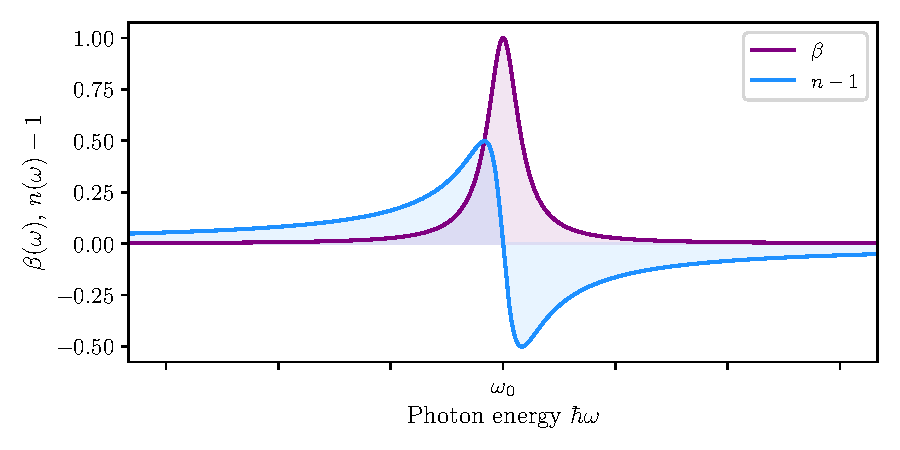
\includegraphics[width=1.0\textwidth]{figures/CATS/KK_example.pdf}
	\caption[Example real and imaginary refractive index calculated using KK relations]{Example real $n(\omega)$ (purple) and imaginary $\beta(\omega)$ (blue) refractive index for a Lorentzian absorption line shape with a resonance at energy $\omega_0$.  The real part was calculated from the imaginary using the KK relation from equation \ref{eqn:KK_n_beta}.}
	\label{fig:KK_example}
\end{figure}



\begin{figure}
	\centering
	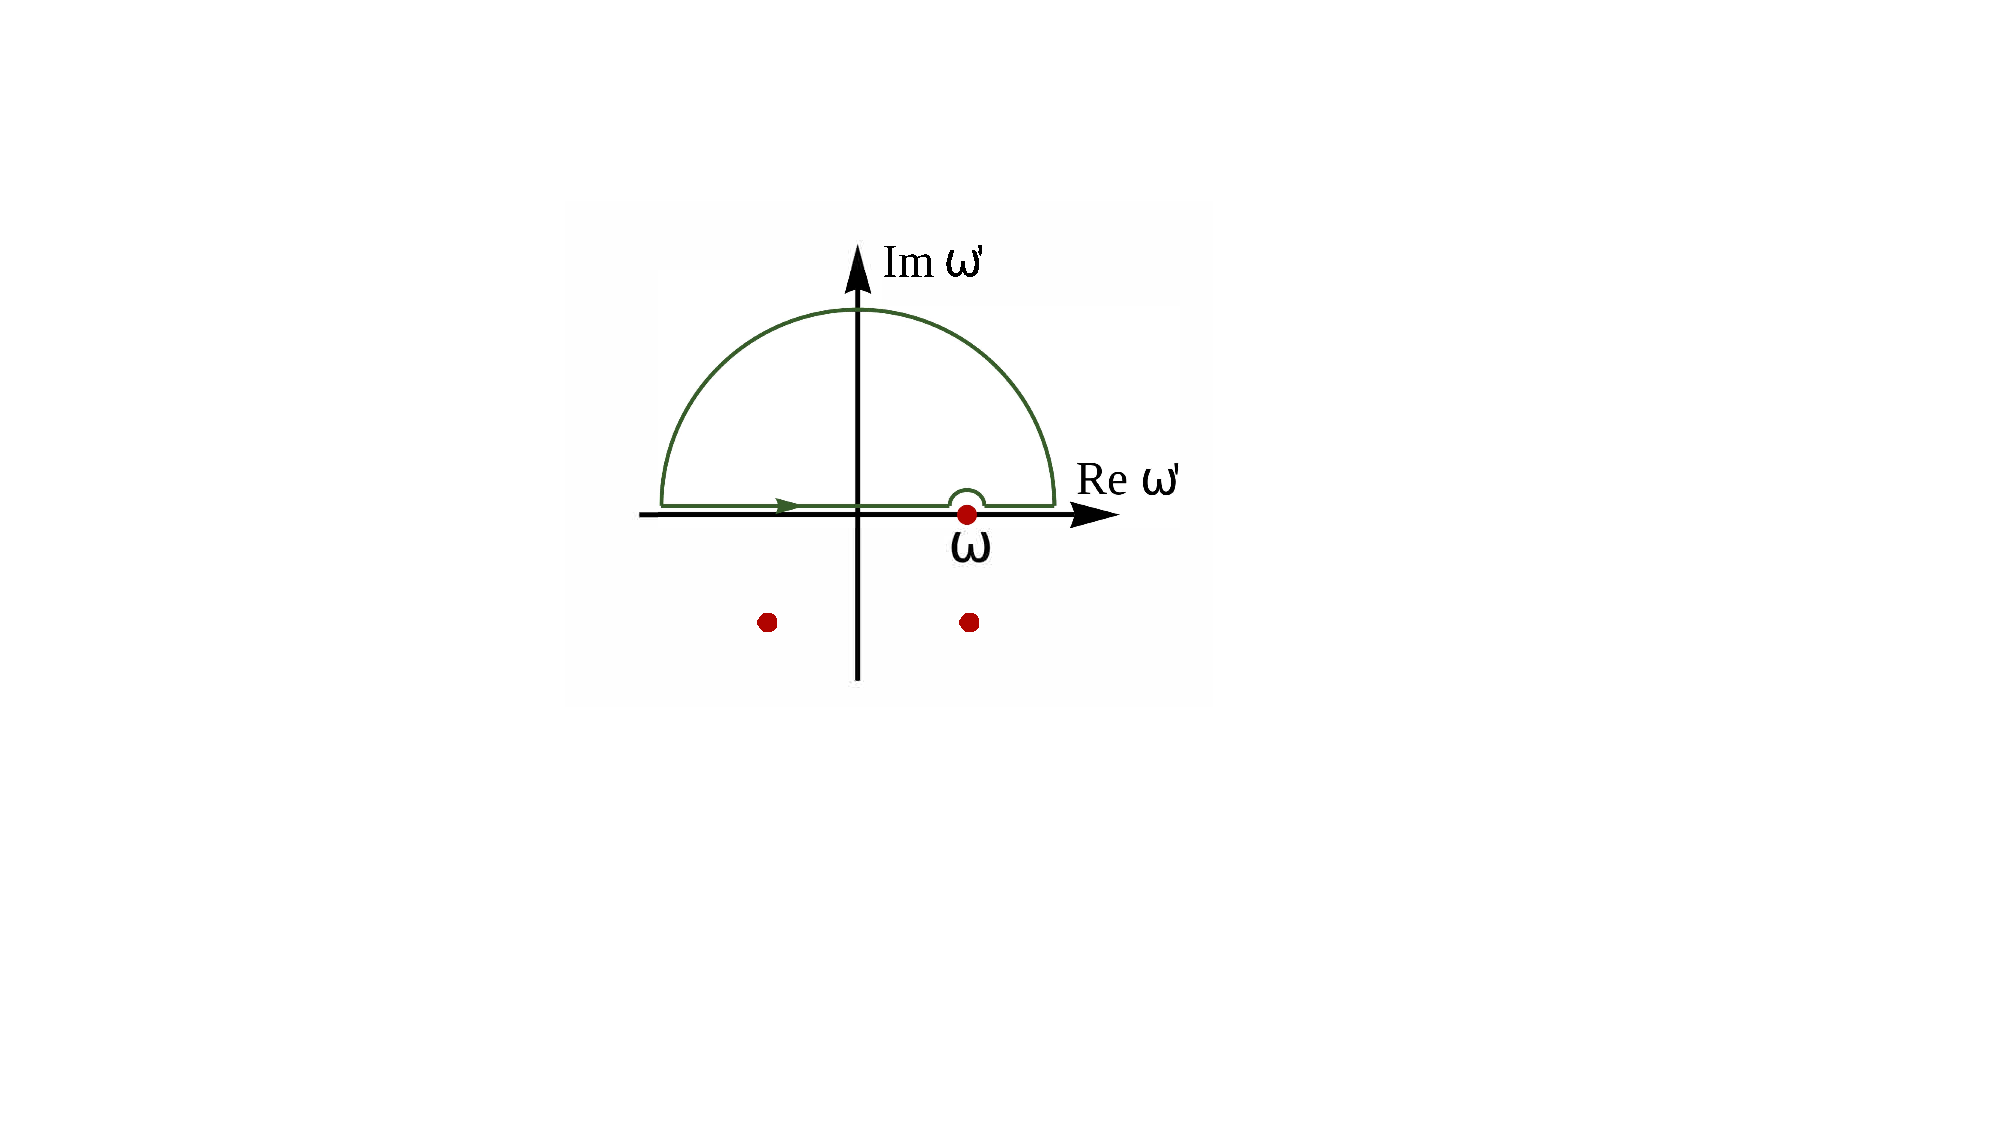
\includegraphics[width=0.4\textwidth]{figures/CATS/KK_no_pump.pdf}
	\caption[Contour used to derive KK relations]{Contour $\Gamma$ (green) in the complex plane of $\omega$ used to derive the KK relations.  Poles are shown in red for the case of a simple harmonic oscillator.}
	\label{fig:KK_contour}
\end{figure}

There is another method to derive the KK relations that is more direct, but it is less physically intuitive \cite{jacksonClassicalElectrodynamics1999, hutchingsKramersKronigRelationsNonlinear1992, lucariniKramersKronigRelationsOptical2005}. This method involves evaluating a contour integral of the susceptibility in the complex plane of $\omega$ for the contour shown in figure \ref{fig:KK_contour}, and this integral is given by 
\begin{equation}
	\label{eqn:contour_int}
	\oint_{\Gamma}\frac{\chi(\omega')}{\omega' - \omega} \diff \omega' = 2\pi i \sum_{k}\mathrm{Res}\big[ \chi(\omega', \omega'_{k}) \big]=0
\end{equation} 
where the residue theorem has been applied and $\mathrm{Res}\big[ \chi(\omega', \omega'_{k}) \big]$ is the residue of $\chi$ at the pole $\omega'_k$.  Since the contour encircles no poles, the sum of residues is zero.  This integral can be broken up into parts consisting of the two arcs and the line across $\mathrm{Re}[\omega']$, and limiting cases can be applied to arrive at equation \ref{eqn:KK_chi},
\begin{equation}
	\chi(\omega)=\frac{1}{i\pi}\mathrm{PV}\int_{-\infty}^{\infty}\frac{\chi(\omega')}{\omega' - \omega}\diff \omega'.
\end{equation}
Though the details of this derivation are not reproduced herein, the key assumption that must be met is that the susceptibility has no poles in one half plane of the complex $\omega$ plane.  Mathematically, this is equivalent to the function $\chi$ being holomorphic \cite{lucariniKramersKronigRelationsOptical2005}.  If $\chi$ has poles in both half planes, then the sum of residues is non-zero and the KK relations do not apply.  As will be shown later, this can happen in certain physical scenarios.

There were some assumptions that were made in the derivation of the KK relation in equation \ref{eqn:KK_n_beta} that are important to scrutinize because they are not generally true.  The first assumption that was made was using the linear susceptibility $\chi(\omega)$.  By doing so we derived the linear KK relations, and these do not hold true when considering higher order nonlinear optical processes \cite{lucariniKramersKronigRelationsOptical2005, hutchingsKramersKronigRelationsNonlinear1992}.  For a higher order process, it is possible to derive KK relations that link the real and imaginary part, and these relations generally take the form given by
\begin{equation}
	\label{eqn:dn_db_KK}
	\Delta\tilde{n}(\omega, \zeta) = \frac{2\omega}{\pi} \mathrm{PV}\int_{0}^{\infty} \frac{\Delta\tilde{\beta}(\omega',\zeta)}{\omega'^2 - \omega^2} \diff \omega'
\end{equation}  
where $\Delta\tilde{n}(\omega, \zeta)$ and $\Delta\tilde{\beta}(\omega,\zeta)$ are the change in the real and imaginary refractive index due to a perturbation $\zeta$ \cite{hutchingsKramersKronigRelationsNonlinear1992, lucariniKramersKronigRelationsOptical2005}.  For an $n$-th order nonlinear process, these changes in the refractive index will generally be proportional to the real and imaginary parts of the $n$-th order nonlinear susceptibility $\chi^{(n)}$ \cite{boydNonlinearOptics2008, lucariniKramersKronigRelationsOptical2005, hutchingsKramersKronigRelationsNonlinear1992}.

Beyond the assumption of the linear susceptibility, another scenario in which the validity of the KK relations must be examined is the case of a pump-probe experiment \cite{tokunagaFemtosecondTimeresolvedDispersion1993, tokunagaFemtosecondContinuumInterferometer1996, lucariniKramersKronigRelationsOptical2005}.  This was examined both theoretically and experimentally by Tokunaga, et. al. \cite{tokunagaFemtosecondTimeresolvedDispersion1993, tokunagaFemtosecondContinuumInterferometer1996}, and this discussion follows from their example.  Consider the change in polarization due to the pump pulse given by
\begin{equation}
	\Delta P(t) = \chi(t)\circledast \big( \mathcal{E}(t) \Delta N(t-\tau)\big) = \int_{0}^{\infty}\chi(t')\mathcal{E}(t-t')\Delta N(t - t' - \tau) \diff t'
\end{equation}
where $\Delta N (t-\tau)$ represents the change in the medium due to the pump pulse for a time delay of $\tau$.  The change in susceptibility now becomes
\begin{equation}
	\label{eqn:d_chi}
	\begin{aligned}
		\Delta\chi(\omega) &= \tilde{\mathcal{E}}(\omega) \mathcal{F}\big[\Delta P(t)\big] = \tilde{\mathcal{E}}(\omega) \mathcal{F}\big[ \chi(t)\circledast \big( \mathcal{E}(t) \Delta N(t-\tau)\big) \big]\\
		& = \frac{\chi(\omega)}{\tilde{\mathcal{E}}(\omega)}\int_{-\infty}^{\infty}\mathcal{E}(t)\Delta N (t-\tau) e^{-i\omega t }\diff t.
	\end{aligned}
\end{equation}
The issue with this change in susceptibility is that within the complex plane of $\omega$ it has poles in both half planes because the integration is over all $t$ \cite{tokunagaFemtosecondTimeresolvedDispersion1993, tokunagaFemtosecondContinuumInterferometer1996, lucariniKramersKronigRelationsOptical2005}.  This presents a problem because when we try to derive the KK relations by evaluating the contour integral over the contour shown in figure \ref{fig:KK_contour_pump}, the sum of residuals is no longer zero.  The residue term is problematic because it requires known of the complex function to evaluate the residue, and this means that you no longer have a simple relationship between the real and imaginary parts.  Therefore, the KK relations do not hold for this case.

\begin{figure}
	\centering
	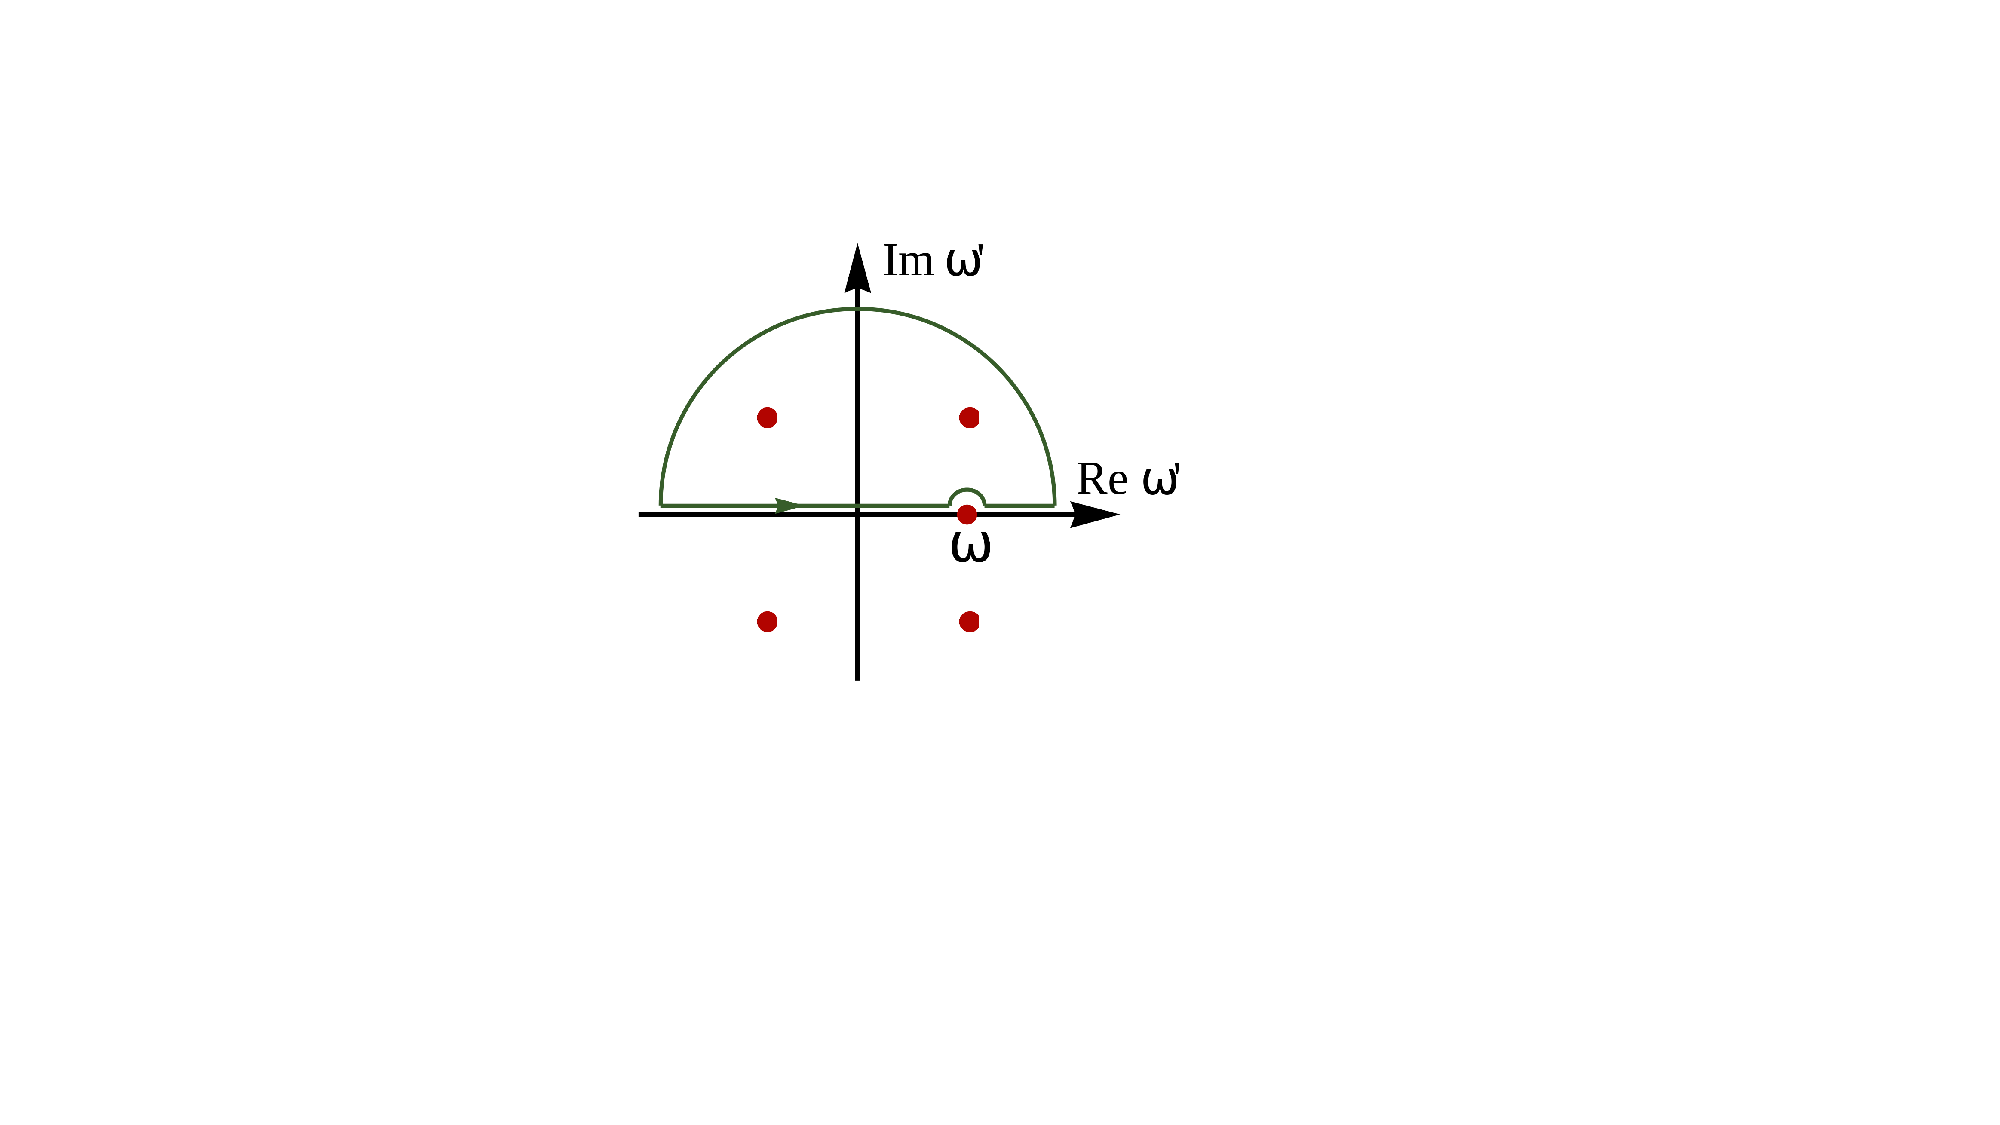
\includegraphics[width=0.4\textwidth]{figures/CATS/KK_pump.pdf}
	\caption[Contour used to derive KK relations in the presence of a pump field]{Contour (green) in the complex plane of $\omega$ used to derive the KK relations.  Poles are shown in red.}
	\label{fig:KK_contour_pump}
\end{figure}

If some assumptions are made about $\Delta N(t-\tau)$, then the KK relations can be recovered. There are four special cases where this is possible \cite{tokunagaFemtosecondTimeresolvedDispersion1993, tokunagaFemtosecondContinuumInterferometer1996}:
\begin{itemize}
	\item $\Delta N(t-\tau)$ is a constant value $\Delta N_0$.  This leads to the change in susceptibility being $\Delta\chi(\omega) = \Delta N_0 \chi(\omega)$. 
	\item $\mathcal{E}(t)$ is a $\delta$-function $\mathcal{E}_0\delta(t)$.  The change of susceptibility is then $\Delta\chi(\omega) = \Delta N (\tau)\chi(\omega)$.
	\item $\Delta N(t)=0$ for $t<0$.  The change of susceptibility is then $\Delta\chi(\omega) = \frac{\chi(\omega)}{\tilde{\mathcal{E}}(\omega)}\int_{0}^{\infty}\mathcal{E}(t)\Delta N (t-\tau) e^{-i\omega t }\diff t$, and there are only poles in the lower half plane.
	\item $\Delta N(t)=0$ for $t>0$.  The change of susceptibility is then $\Delta\chi(\omega) = \frac{\chi(\omega)}{\tilde{\mathcal{E}}(\omega)}\int_{-\infty}^{0}\mathcal{E}(t)\Delta N (t-\tau) e^{-i\omega t }\diff t$, and there are only poles in the upper half plane.
\end{itemize}
Each of these special cases allows for the KK relations to be satisfied, however the last case actually means that the KK relations have the opposite sign.  As a demonstration, Tokunaga et. al. experimentally tested these cases by performing a pump/probe experiment using a femtosecond frequency-domain interferometer to simultaneously measure both the real and imaginary parts of the refractive index \cite{tokunagaFemtosecondTimeresolvedDispersion1993}.  What they found was that the KK relations were valid at most delays, however the KK relations were not valid at temporal overlap between their pump and probe pulse.  This can be seen evidently in the data because the real and imaginary parts have the same symmetry, and this clearly violates the KK relations.

The breakdown of the KK relations in certain cases means that they have to be cautiously applied to pump/probe experiments, such as in ATS.  There have been recent experiments that used the Fourier transform implementation of the KK relations \cite{petersonCausalityCalculationsTime1973} to indirectly calculate the real part from the experimentally measured change in absorption \cite{stoossRealTimeReconstructionStrongFieldDriven2018}.  In that case, the KK relations are expected to be valid because their XUV pulse was an IAP (approximately a $\delta$-function), and they limited their investigations to only a single time delay point that corresponded to the IR dressing field arriving after the XUV pulse.  These limitations highlight the challenges that are presented by relying on an indirect calculation to reconstruct the real and imaginary parts.  This is one of the reasons that a direct measurement is generally preferable because there are less assumptions that have to be made about the underlying dynamics that are of interest.  To this end, the CATS technique represents a new method to directly measure both part of the refractive index change, and this will be demonstrated experimentally in the following section.




\section{Complex Attosecond Transient-absorption Spectroscopy of Fano resonances}
\label{sec:CATS_ar}

Now that the principle behind the CATS technique using a SWPG was established, in this section an experimental demonstration will be discussed.  The system of interest is the same as in Chapter \ref{chap:ATS}, the $3s3p^6np$ Argon Fano resonances in the presence of an IR dressing field. This was done in an effort to examine the same physical scenario using both the traditional ATS method and the new CATS method.

\subsection{Experimental setup}
\label{sec:CATS_ar_exp_setup}

The experimental setup to demonstrate the CATS method is similar to the setup in Chapter \ref{chap:ATS}, and it is shown schematically in figure \ref{fig:CATS_setup}.  The primary differences between the two setups are the obvious presence of the SWPG to generate two XUV sources and the removal of the second harmonic generation optics that were used generate even and odd  high harmonics.  The dressing arm of the TABLe interferometer remains unchanged between the two experiments, and this allows for dressing of the gas sample with an intensity up 35 TW/cm$^2$ at a wavelength of 1435 nm and a nominal pulse duration of 60 fs. The spot size of the dressing beam is 34 $\mu$m in diameter, and this allows for the dressing of only one of the two XUV sources in that propagate through the gas cell in the target chamber.

\begin{figure}
	\centering
	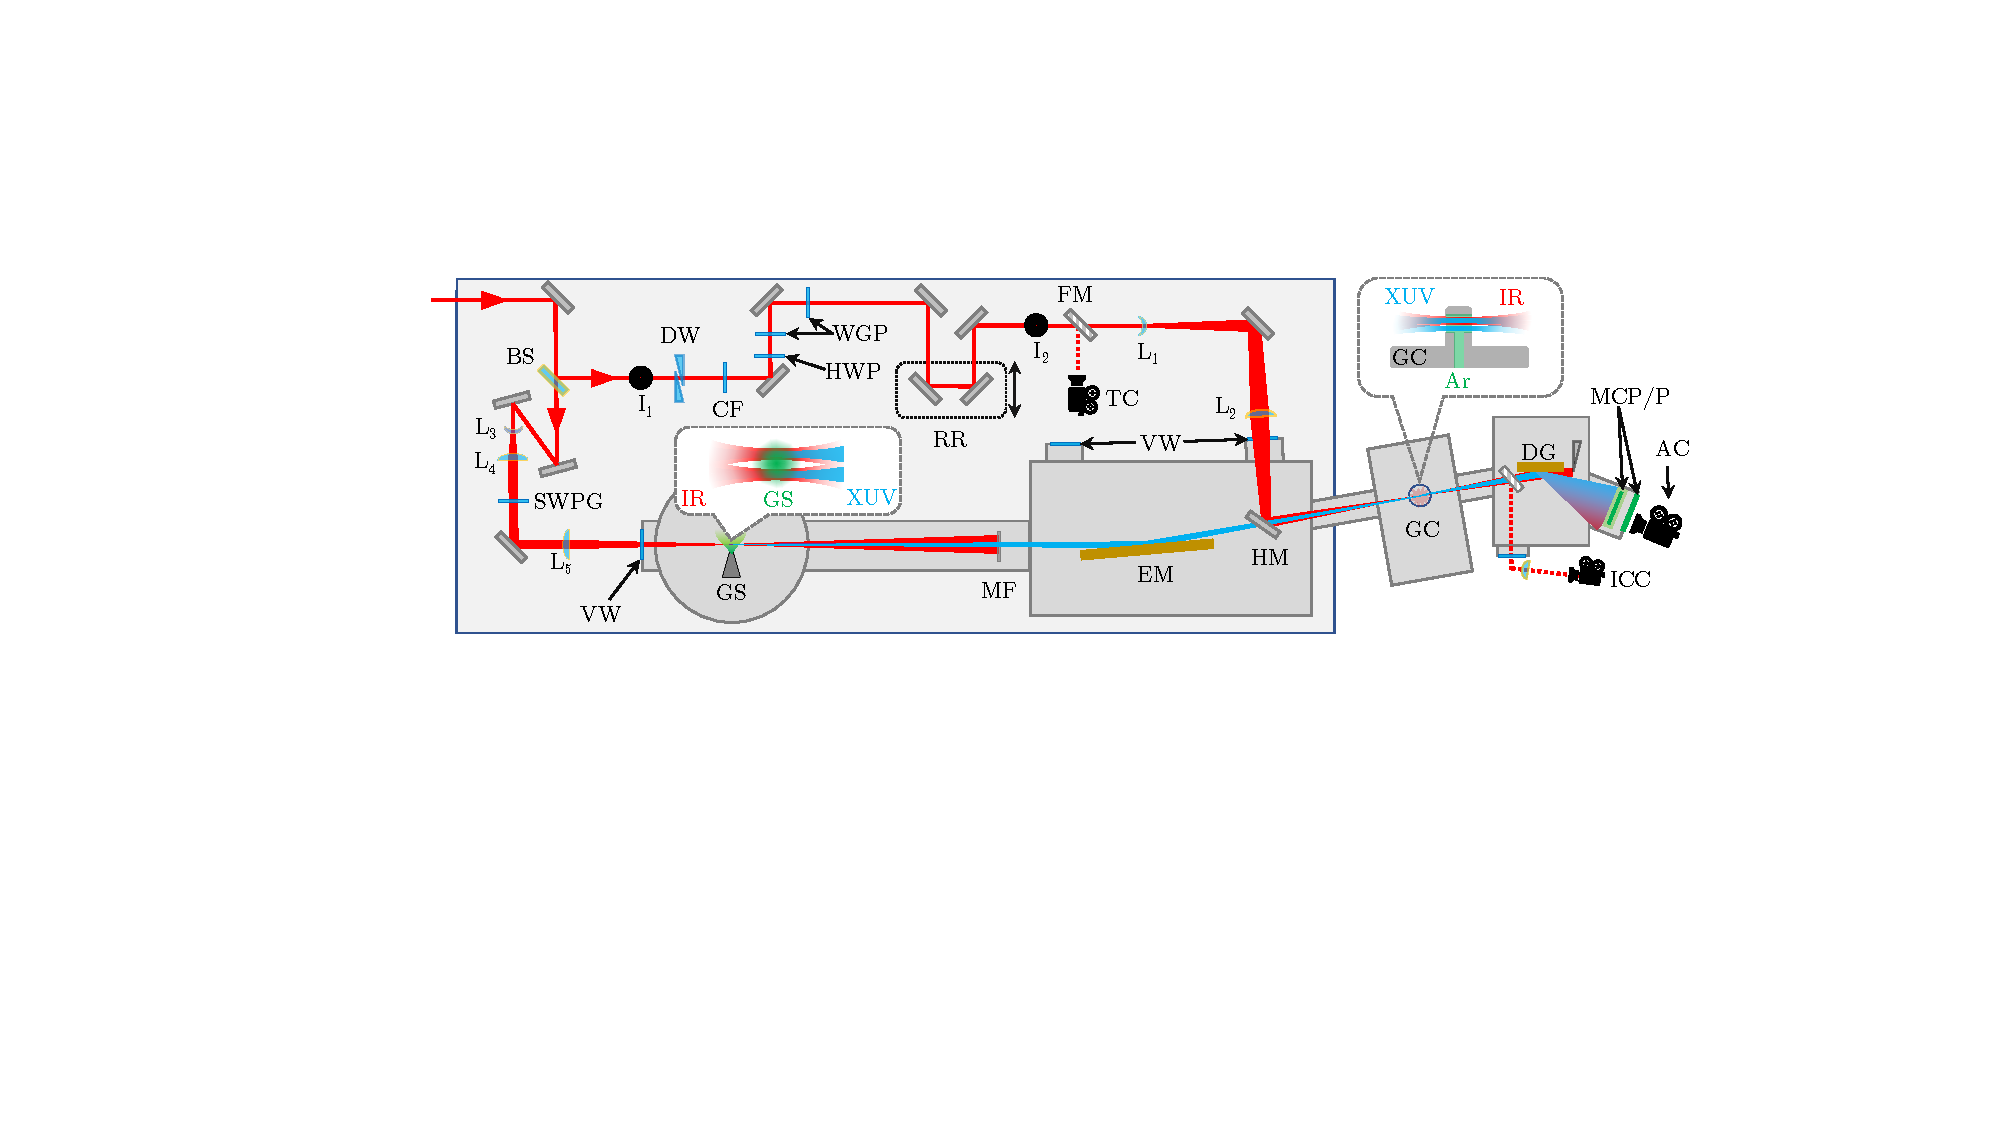
\includegraphics[width=1.0\textwidth]{figures/CATS/beamline_schematic_CATS.pdf}
	\caption[TABLe experimental setup for CATS experiments]{Schematic of the optical setup for the experiments described in this chapter.  Insets show the two-source harmonic generation using the SWPG and the dressing of only one of the two XUV sources by an IR dressing field.  \textbf{BS}: Beamsplitter, \textbf{I$_{1,2}$}: Irises used for alignment. \textbf{DW}: Delay wedges for fine delay control. \textbf{CF}: Color filter. \textbf{HWP}: Half-wave plate. \textbf{WGP}: Wire grid polarizer. \textbf{RR}: Retro reflector for coarse delay adjustment.  \textbf{FM}: Flip mirror. \textbf{TC}: Thermal camera used for alignment.  \textbf{L$_1$}: $f=-300$ mm lens. \textbf{L$_2$}: $f=500$ mm lens. \textbf{VW}: Vacuum window, \textbf{HM}: Hole mirror with 10 mm hole.  \textbf{L$_3$}: $f=-400$ mm lens.  \textbf{L$_4$}: $f=500$ mm lens. \textbf{L$_5$}: $f=400$ mm lens. \textbf{SWPG} $0-\pi$ square-wave phase grating. \textbf{GS}: Gas source for HHG. \textbf{MF}: Aluminum filter. \textbf{EM}: Ellipsoidal mirror. \textbf{GC}: Gas cell. \textbf{RM}: Removable mirror for \textit{in-situ} diagnostics.    \textbf{ICC}: camera for \textit{in-situ} diagnostics. \textbf{DG}: VLS diffraction grating. \textbf{MCP/P}: Microchannel plate and phosphor.  \textbf{AC}: Andor Neo 5.5 CMOS camera.}
	\label{fig:CATS_setup}
\end{figure}

In order to dress only one of the two XUV sources in the target chamber, as is shown in the inset of figure \ref{fig:CATS_setup}, the hole mirror is titled to achieve spatial overlap with only one source.  This overlap between the dressing and one XUV sources was verified by placing a camera at the focal plane within the target chamber.  The disadvantage of this method for spatial alignment between the dressing and the XUV source is that there is now an angle introduced between the two wave fronts at the focal plane of the XUV.  This angle is given by
\begin{equation}
	\theta = \tan^{-1}\bigg(\frac{\Delta x}{6 D}\bigg) = \tan^{-1}\bigg(\frac{\lambda f}{3 d D}\bigg)
\end{equation}
where $\Delta x = 2\lambda f /d$ is the source separation set by the SWPG of period $d$ for a focal length $f$ and $D$ is the distance between the hole mirror at the focal plane of the XUV. For a SWPG period $d=2.5$ mm, a focal length of $f=400$ mm, and a wavelength of 1435 nm, this corresponds to an angle of 0.139 mrad.  This angular deviation between the two wave fronts accounts for a temporal averaging of 213 as between the XUV and the IR pulses.  This averaging could be avoided in future experiments by adjusting the dressing arm focal geometry to translate the beam instead of just pointing it using a single mirror.

\begin{figure}
	\centering
	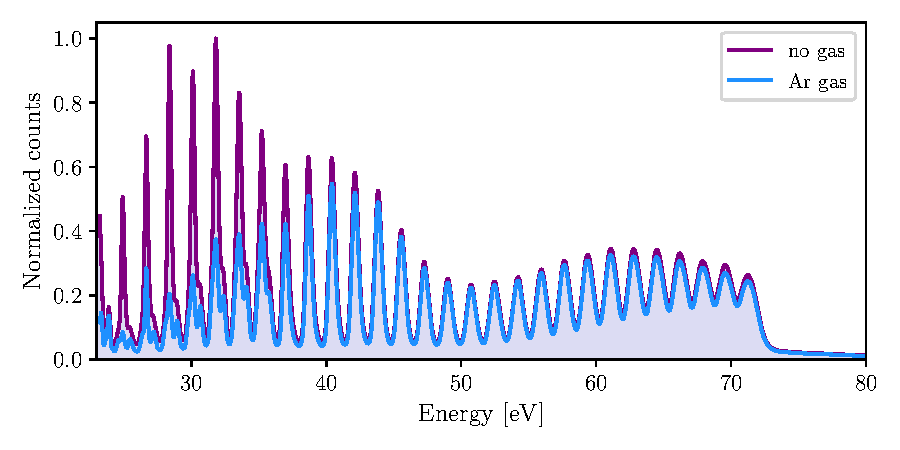
\includegraphics[width=0.9\textwidth]{figures/CATS/ref_harmonic_spectrum.pdf}
	\caption[Reference harmonic spectrum used in CATS experiment]{Reference harmonic spectrum used in CATS experiment with (blue) and without (purple) Ar gas present.}
	\label{fig:ref_harmonic_spectrum}
\end{figure}

As mentioned previously, harmonic generation for this experiment is done at 1435 nm in Ar with a SWPG to generate two sources of XUV.  An example of the harmonic spectrum generated by this setup is shown in figure \ref{fig:ref_harmonic_spectrum}, and only harmonics below 72 eV are seen because a 200 nm aluminium metallic filter is used to filter out the fundamental field used for HHG.  Additionally, in this figure the absorption from the sample Ar gas is shown. To do this, a gas cell is used that is 2 mm in length, 750 $\mu$m in height, and 250 $\mu$m in width.  This cell was selected to allow for both XUV sources to pass through the gas cell.  For the experiments described herein, the backing pressure of the gas cell was set at 62 Torr.  This interaction pressure was similar to the interaction pressure used for the experiments in Chapter \ref{chap:ATS}.

\begin{figure}
	\centering
	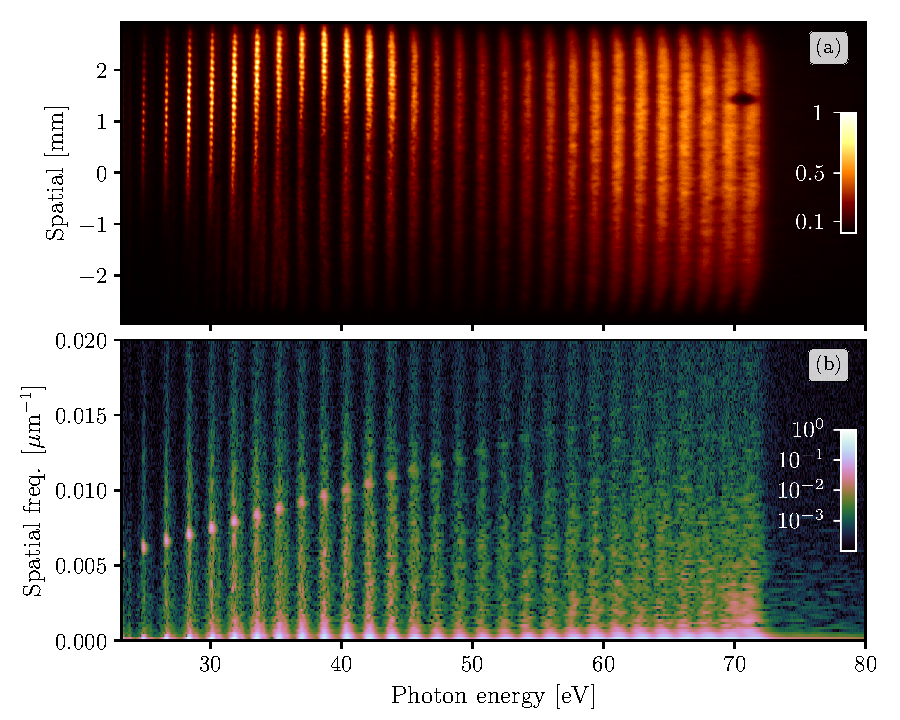
\includegraphics[width=0.9\textwidth]{figures/CATS/ref_image_FFT.pdf}
	\caption[Reference camera image and spatial Fourier transform used in CATS]{(a) Reference image of spectrometer output.  Fringes along the spatial dimensions are due to interference between the two XUV sources generated by the SWPG. (b) Amplitude of Fourier transform along the spatial dimension. Peaks correspond to the spatial frequency of each harmonic order.  Linear dependence of spatial frequency on photon energy is observed.}
	\label{fig:ref_image_FFT}
\end{figure}

To perform this experiment, it is necessary to use a SWPG to generate two XUV sources that can be interfered to act as an inline Mach-Zehnder interferometer.  The details of the SWPG can be found in Chapter \ref{chap:two_source}, and in this case the SWPG that was used had a grating period of $d=2.5$mm.  This entails the the source separation in the generation chamber is 459 $\mu$m for a focal length of 400 mm and a wavelength of 1435 nm.  In the target chamber the source separation is reduced by a factor of 3 due to the demagnification of the ellipsoidal mirror, thus the source separation in the gas cell is only 153 $\mu$m.  An example of the harmonics generate using this setup is shown in figure \ref{fig:ref_image_FFT} (a), and the corresponding amplitude of the Fourier transform along the spatial dimension of the harmonics is shown in figure \ref{fig:ref_image_FFT} (b).  In this Fourier amplitude, clear peaks can be observed at spatial frequencies that correspond to the harmonic order of each harmonic.  This depends linearly with harmonic order, as was discussed in Chapter \ref{chap:two_source}.  The amplitude and phase of each of these peaks will be used to define the fringe contrast and the fringe shift when comparing the harmonic spectra with and without the dressing field present.  This is done in the same manner as was done in Chapter \ref{chap:refractive_index} where the change in fringe contrast and shift was due the presence of a solid sample, however in this case the change in fringe contrast and shift is due the presence of a dressing field. 

\subsection{Results}
\label{sec:CATS_ar_results}

Now that the theoretical background and experimental setup has been thoroughly established, attention can be turned to the experimental results.  The delay dependent change in real and imaginary parts of the refractive index will be shown for both moderate and high dressing field intensities, and the extracted dipole amplitude and phase will be shown. Additionally, the applicability, or lack thereof, of the KK relations will be examined.

To begin, the delay dependent results are shown in figure \ref{fig:delay_high_low} for dressing intensities of 12 TW/cm$^2$ and 33 TW/cm$^2$. In figures \ref{fig:delay_high_low} (a) and (b), the $\dod$ is calculated in a similar manner as was done in Chapter \ref{chap:ATS}  and is comparable to the results that were presented previously. The primary difference between this calculation and what was shown previously is the fact that only one of the two sources being dressed needs to be accounted for to correctly extract the amplitude of the $\dod$ signal.  If the ratio of the total power in each source is $R=I_1/I_2$, then the true change in transmission $\Delta T$ induced by the dressing field can be written in terms of the measured change in total transmission $\Delta \tilde{T}$ as
\begin{equation}
	\label{eqn:dod_fringe_shift}
	\Delta \tilde{T} = \frac{I_1 + \Delta T I_2}{I_1 + I_2} = \frac{R + \Delta T}{1+ R}.
\end{equation}
Using this relationship the true $\dod(\omega)$ is given by 
\begin{equation}
	\label{eqn:dod_R}
	\begin{aligned}
		\dod(\omega) & = -\log(\Delta T(\omega)) = -\log((1+R)\Delta \tilde{T}(\omega) - R) \\
		&= -\log\bigg((1+R)\frac{I_{\mathrm{on}}(\omega)}{I_{\mathrm{off}}(\omega)} - R\bigg)
	\end{aligned}
\end{equation}
where $I_{\mathrm{on}}$ and $I_{\mathrm{off}}$ is the harmonic amplitude with and without the dressing field, respectively.  This ratio $R$ is a free parameter that is used to account for the difference in amplitude between the two sources, and it is generally found to be around $R=0.8$.  To calculate the harmonic amplitude $I_{\mathrm{on,off}}(\omega)$, the spatial profile of the harmonics is integrated over to yield the amplitude as a function of energy.

As can be seen in the $\dod$ in figures \ref{fig:delay_high_low} (a) and (b), there are two main features that can observed at 26.6 eV and 28.5 eV.  These features correspond to the $3s3p^6np$ autoionizing (Fano) resonances for $n=4$ at 26.6 eV and $n=6$ at 28.5 eV, which have been extensively explained in section \ref{sec:fano_ar}.  For this particular experiment, only these two resonances are observed because the harmonic comb that was used only consisted of odd harmonics, as opposed to a comb of even and odd harmonics that can act as a pseudo-continuum of energies if each harmonic has sufficient bandwidth, see section \ref{sec:ATS_ar_exp_setup}.  Thus, only features that are present within the bandwidth of each harmonic can be observed in this experiment.  Consequently, the wavelength of 1435 nm was selected to place two resonances within the bandwidth of neighboring harmonics.

\begin{figure}
	\centering
	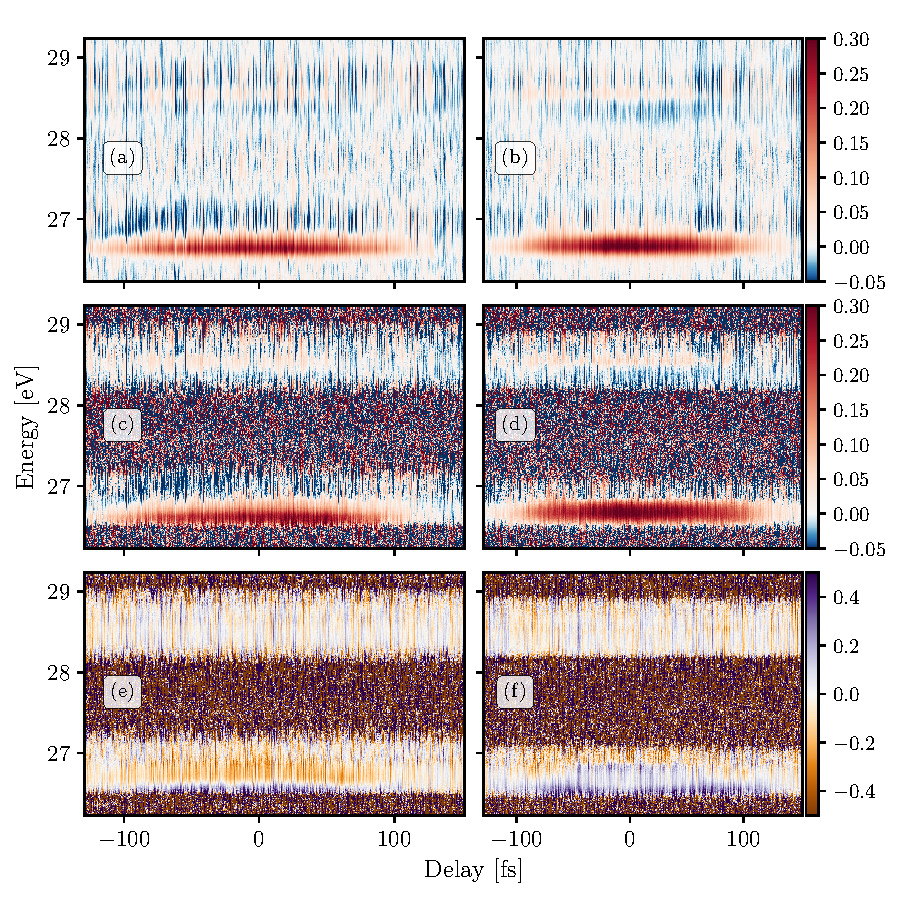
\includegraphics[width=1.0\textwidth]{figures/CATS/delay_high_low.pdf}
	\caption[Delay-dependent $\dod$ and $\Delta \phi$ measured at high and moderate dressing intensities]{(a),(b) $\dod$ calculated when ignoring spatial structure of harmonics.  (c),(d)  $\dod$ calculated using the change in fringe contrast induced by the dressing field.  (e),(f) Phase shift $\Delta\phi\propto\Delta n $ calculated from the fringe shift induced by the dressing field.  Figures on left correspond to a dressing intensity of 12 TW/cm$^2$, and figures on the right correspond to a dressing intensity of 33 TW/cm$^2$.}
	\label{fig:delay_high_low}
\end{figure}

The general interpretation of these features in the $\dod$ was explored in terms of dipole control model (DCM) and Floquet theory in sections \ref{sec:DCM} and \ref{sec:LIS_Floquet}.  Generally speaking, the DCM explains the attenuation and phase shift of the dipole in the time domain due to the influence of the dressing field, and the Floquet theory explains the presence of light-induced states (LIS) that appear in the $\dod$.  For the dressing intensities used in this experiment, the dipole is strongly suppressed by the dressing field, as was shown in the intensity dependence of the $\dod$ in figures \ref{fig:dOD_HWP} and \ref{fig:np_intensity_dep}.  The Floquet theory accounts for the presence of LIS in the absorption spectrum that are generally observed between the bright $np$ resonances.  In this case, since we can only observed changes within the bandwidth of each harmonic, the same LISs are not observed.  However, Floquet theory should still be able to account for the shifting of levels in the dressed atom picture.  The observed delay dependent $\dod$ is consistent with what was observed previously, see section \ref{sec:ATS_ar_delay}, and the primary difference being that only features near the bright $4p$ and $6p$ states is observed.

Moving beyond the typical ATS measurement, in figures \ref{fig:delay_high_low} (c) and (d) the change in fringe contrast is used to extract the $\dod$.  This is done by Fourier transforming the spatial structure of the harmonics and taking the amplitude of the spatial frequency corresponding to the harmonic energy.  From this, the fringe contrast $V$ is defined as
\begin{equation}
	V=\frac{I_{\mathrm{max}} - I_{\mathrm{min}}}{I_{\mathrm{max}} + I_{\mathrm{min}}} = \frac{I_{\mathrm{amp}}}{I_{\mathrm{mean}}}.
\end{equation}
If $V$ ($V_0$) is the contrast with (without) the dressing field, then the imaginary part $\Delta\beta$ can be calculated using equation \ref{eqn:beta_fringe_contrast_chap_cats}.  From this, the $\dod$ can then be calculated using equation \ref{eqn:dod_to_beta}, and this is exactly what is shown in figures \ref{fig:delay_high_low} (c) and (d) for a dressing intensity of 12 TW/cm$^2$ and 33 TW/cm$^2$, respectively.  Comparing the $\dod$ extracted using this method and the typical method, it can be seen that there is overall good agreement between the two methods.  The primary difference is that extracting the $\dod$ using the fringe contrast can only be done where the fringe visibility is sufficiently high within the bandwidth of each harmonic.  This limits the energy range that can be used to extract the $\dod$, however it still represents a significant fraction of the harmonic bandwidth.

The more interesting component of this measurement is shown in figures \ref{fig:delay_high_low} (e) and (f), which are the phase shift $\Delta\phi$ as a function of energy and delay that is extracted from the fringe shift of the spatial interference pattern.  This is done in similar manner as the $\dod$ by Fourier transforming the spatial structure of the harmonics and taking the phase of the spatial frequency corresponding to that harmonic energy.  The difference in this phase with and without the dressing field gives the dressing field induced phase shift $\Delta\phi$ that is proportional to the real part of the refractive index $\Delta n$, see equation \ref{eqn:phase_shift_dn}.  As can be seen, there is a clear delay dependent phase shift that confirms the feasibility of measuring both parts of the refractive index using CATS. 

\begin{figure}
	\centering
	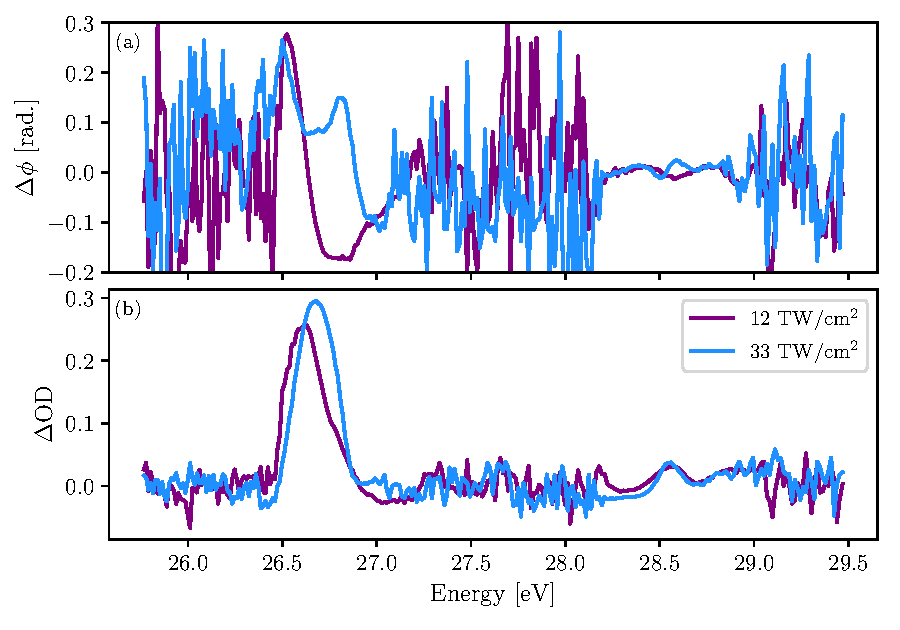
\includegraphics[width=0.9\textwidth]{figures/CATS/dphi_dod_lineout.pdf}
	\caption[Line outs of $\Delta\phi$ and $\dod$ for $\tau=0$ using CATS]{(a) Line outs of the dressing field induced phase $\Delta\phi$ for the two intensities 12 TW/cm$^2$ (purple) and 33 TW/cm$^2$ (blue).  (b) Line outs of the $\dod$ measured using the dressing field induced change in fringe contrast for the two intensities.}
	\label{fig:dphi_dod_lineout}
\end{figure}

Additionally, in the delay dependent phase shift $\Delta\phi$ there is a clear difference in the induced phase between the two intensities.  To examine this further, it is useful to look at line outs along the energy axis for a delay corresponding to $\tau=0$, and this is shown in figure \ref{fig:dphi_dod_lineout}.  At the lower intensity, the phase shift in the vicinity of the $4p$ resonance has an asymmetric dispersive line shape.  However, at the higher intensity the structure of the phase difference is more complicated.  On the low energy side near 26.5 eV there is agreement between the two intensities, however a second peak appears at 26.8 eV.  This second peak can attributed to a LIS based upon its energy because it is separated by approximately $2\omega=1.74$  eV from the higher $6p$ resonance at 28.5 eV.  The fact that this transition would be three photons (1 XUV - 2 IR) from the ground state means that it would depend strongly on the dressing intensity \cite{shankarPrinciplesQuantumMechanics2013}, and thus it would only be expected to appear at the higher dressing intensity near temporal overlap between the XUV and IR pulses.  This is exactly what is observed in figure \ref{fig:delay_high_low}. At higher energies near the $6p$ resonance, there is also a clear difference in the induced phase between the two intensities.  At lower intensities there is a broad decrease in phase difference, however at higher intensities this becomes more of a dispersive line shape and changes sign.

In terms of the $\dod$ line outs shown in figure \ref{fig:dphi_dod_lineout} (b), there is also a clear difference between the two intensities that were measured.  Near the $4p$ resonance the line shape for both intensities is qualitatively similar because there appears to be only a single peak for both intensities, however the peak position and shape is different between the two cases.  The higher intensity case shows the peak shifted to higher energies, and this can most likely be attributed to the presence of an unresolved peak in $\dod$ due to the LIS that was observed in the induced phase difference.  Near the $6p$ resonance there is less of a difference between the two intensities.  Generally speaking, they have the same shape, however the higher intensity case shows a slightly narrower peak.

\begin{figure}
	\centering
	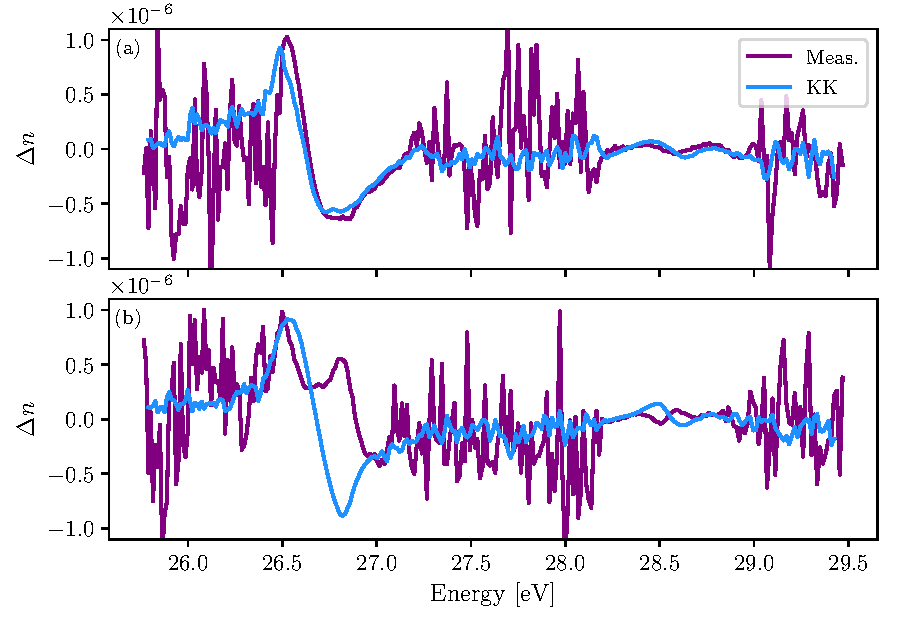
\includegraphics[width=0.9\textwidth]{figures/CATS/dn_kk_lineout.pdf}
	\caption[Nonlinear KK relation applied to CATS measurement]{Indirect calculation of $\Delta n$ using the nonlinear KK relation for (a) the lower intensity of 12 TW/cm$^2$ and (b) the higher intensity 33 TW/cm$^2$.}
	\label{fig:dn_kk_lineout}
\end{figure}

Now that the phase difference $\Delta\phi$ and the change in absorption $\dod$ has been characterized, one question to ask is: can this same result be achieved using only the KK relations? To explore this option, the nonlinear KK relation given by equation \ref{eqn:dn_db_KK} is used to indirectly calculate the change in real refractive index $\Delta n = \lambda \Delta\phi/2\pi L$, and this is shown in figure \ref{fig:dn_kk_lineout}.  For the lower intensity the answer appears to be yes, the KK relations can be applied in this case to indirectly calculate the real part from the imaginary.  The primary difference between the calculation and the experimental values is near the $6p$ resonance where the shape is reproduced, but the peak positions are slightly shifted.  This is most likely due to the small signal in this region that is close to the noise floor.  That being said, the story is quite different at higher intensities.  In this case, the KK relation completely fails to reproduce the experimental data.  The peak near 26.5 eV is reasonably reproduced, however the LIS peak at 26.8 eV cannot be reproduced by the KK relation.  Additionally, the features seen near the $6p$ resonance at 28.5 eV has the opposite sign.  The failure of the KK relations is not surprising in this case because they fundamentally connect shapes of opposite symmetry, and the fact the $\dod$ was symmetric for both intensities means that it can only produce and asymmetric line shape for the real part.  This break down of the KK relations near overlap has been experimentally observed before \cite{tokunagaFemtosecondTimeresolvedDispersion1993}.  However, the intensity dependent breakdown of the KK relation will require more theoretical effort to fully understand.

\begin{figure}
	\centering
	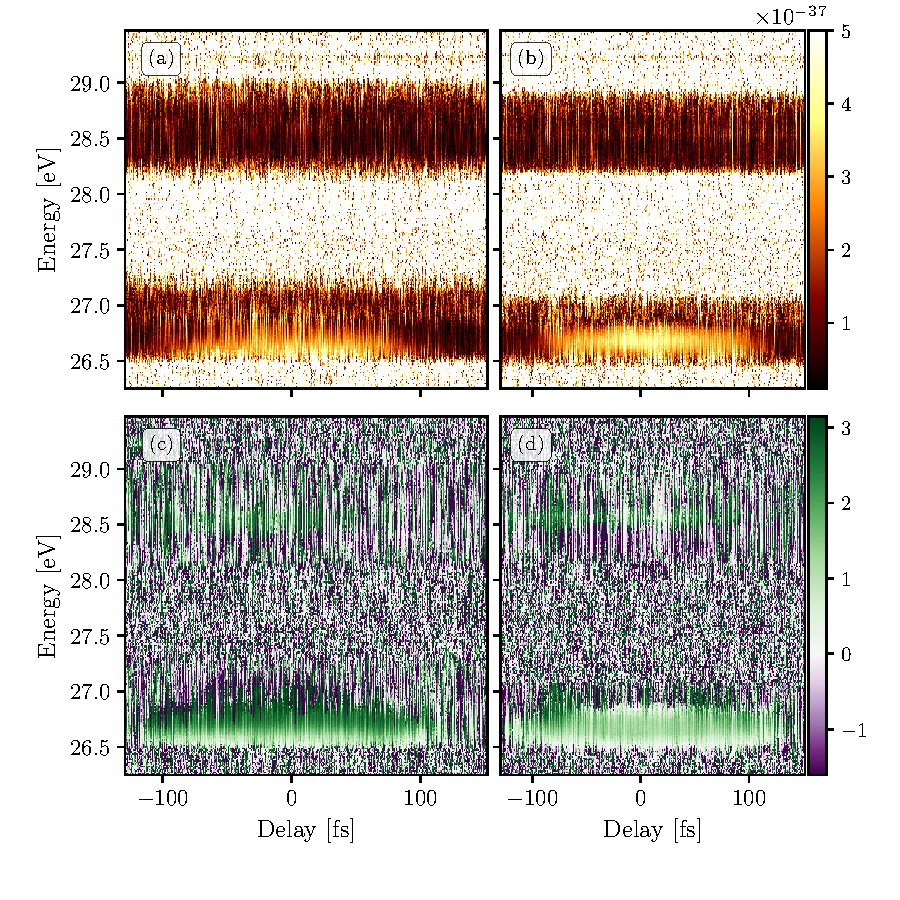
\includegraphics[width=1.0\textwidth]{figures/CATS/amp_ph_delay.pdf}
	\caption[Polarizability amplitude and phase extracted from CATS measurement for two dressing intensities]{(a),(b) Amplitude of change in polarizability $\Delta\alpha$ in units of Fcm$^2$. (c),(d) Phase of change in polarizability $\Delta\alpha$ in units of rad.  Figures on left correspond to a dressing intensity of 12 TW/cm$^2$m, and figures on right correspond to a dressing intensity of 33 TW/cm$^2$.}
	\label{fig:amp_ph_delay}
\end{figure}

\begin{figure}
	\centering
	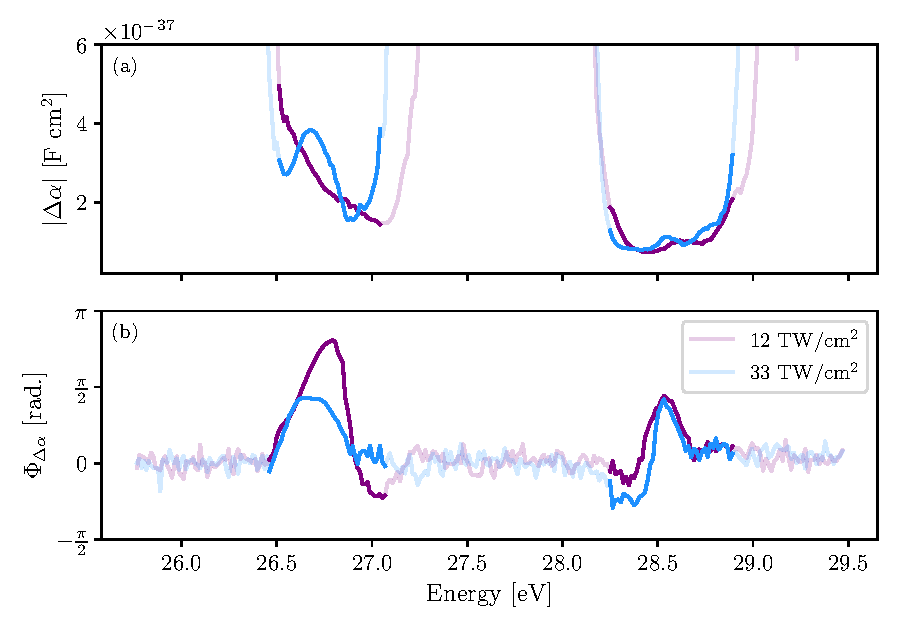
\includegraphics[width=0.9\textwidth]{figures/CATS/amp_ph_lineout.pdf}
	\caption[Line outs of $\lvert\Delta\alpha\rvert$ and $\Phi_{\Delta\alpha}$ at $\tau=0$ using CATS]{(a) Line outs of $\lvert\Delta\alpha\rvert$ at temporal overlap, $\tau=0$, for dressing intensities of 12 TW/cm$^2$ (purple) and 33 TW/cm$^2$ (blue). (b) Line out of the phase $\Phi_{\Delta\alpha}$ for the two intensities.  The greyed out lines indicate where the harmonic amplitude was zero, and therefore the extracted values are not meaningful.}
	\label{fig:amp_ph_lineout}
\end{figure}

A final feature that can be extracted using CATS is the amplitude and phase of the dipole from these measurements.  In order to extract the dipole, knowledge of the electric field $\tilde{\mathcal{E}}(\omega)$ sprectral amplitude and phase needs to be known.  This can be seen in the relationships given by equations \ref{eqn:dn_re_dipole} and \ref{eqn:dod_im_dipole}.  The amplitude is directly measured in the experiment, however the phase in unknown.  In principle, the phase can be measured using RABBITT \cite{paulObservationTrainAttosecond2001}, or it could be calculated \cite{lewensteinTheoryHighharmonicGeneration1994}.  In lieu of that, the change in polarizability can be extracted, where the polarizability is given by $\alpha=\tilde{d}/\tilde{\mathcal{E}}$.  Thus, the amplitude of $\Delta\alpha$ is given by
\begin{equation}
	\label{eqn:polariz_amp}
	\lvert\Delta\alpha\rvert^2 = \Bigg(\frac{2\epsilon_0}{g\rho}\Delta n\Bigg)^2 + \Bigg( \frac{\epsilon_0 c \ln 10}{g \rho \omega L}\dod \Bigg)^2,
\end{equation}
and the phase of $\Delta\alpha$ is given by
\begin{equation}
	\label{eqn:polariz_phase}
	\Phi_{\Delta\alpha}=\arg\Bigg[ \frac{2\epsilon_0}{g\rho}\Delta n  + i \frac{\epsilon_0 c \ln 10}{g \rho \omega L}\dod\Bigg].
\end{equation}
The change in amplitude and phase of $\Delta\alpha$ is shown in figure \ref{fig:amp_ph_delay} for the two intensities.  To highlight the differences between the two intensities, line outs of $\lvert\Delta\alpha\rvert$ and $\Phi_{\Delta\alpha}$ near temporal overlap is shown in figure \ref{fig:amp_ph_lineout}.  




\section{Conclusion}
\label{sec:CATS_conclusion}
In this chapter, the change in real and imaginary refractive index was expounded theoretically to motivate the need for a new method to measure the complex refractive index in a transient absorption experiment.  The method developed to do this is Complex Attosecond Transient-absorption Spectroscopy (CATS).  CATS leverages a 0-$\pi$ SWPG to generate a reference XUV field that can be used to measure both parts of the refractive index.  This method was verified experimentally by studying the Argon Fano resonances in the presence of a IR dressing field of moderate and high intensity.  The demonstration of CATS allows for the direct measurement of the complex refractive index in a host experiments, and paves the way for future research by measuring a feature that was previously only indirectly accessible in typical ATS experiments. 


